% ---------------------------------------------------------------------------
% Author guideline and sample document for EG publication using LaTeX2e input
% D.Fellner, v1.13, Jul 31, 2008

\documentclass{egpubl-eurovis-star}
\usepackage{eurovis2014-star}

% --- for EuroVis
%\WsSubmission    % uncomment for submission to EuroVis
\WsPaper         % uncomment for final version of EuroVis contribution

\electronicVersion % can be used both for the printed and electronic version

% !! *please* don't change anything above
% !! unless you REALLY know what you are doing
% ------------------------------------------------------------------------

% for including postscript figures
% mind: package option 'draft' will replace PS figure by a filname within a frame
\ifpdf \usepackage[pdftex]{graphicx} \pdfcompresslevel=9
\else \usepackage[dvips]{graphicx} \fi

\PrintedOrElectronic

% prepare for electronic version of your document
\usepackage{t1enc,dfadobe}

\usepackage{egweblnk}
\usepackage{cite}

% For backwards compatibility to old LaTeX type font selection.
% Uncomment if your document adheres to LaTeX2e recommendations.
% \let\rm=\rmfamily    \let\sf=\sffamily    \let\tt=\ttfamily
% \let\it=\itshape     \let\sl=\slshape     \let\sc=\scshape
% \let\bf=\bfseries

% end of prologue

%\input{EGauthorGuidelines-body.inc} % commented by KK for ShareLaTeX use

% ---------------------------------------------------------------------
% EG author guidelines plus sample file for EG publication using LaTeX2e input
% D.Fellner, v1.17, Sep 23, 2010


\title[EG \LaTeX\ Author Guidelines]%
      {Bridge and terrain reconstruction in LiDAR point clouds}

% For anonymous conference submission, please enter your SUBMISSION ID.
\author[submission ID]{Timotej Kovač}

%% For the final version of your accepted paper, please enter the authors names and affiliations.
%\author[D. Fellner \& S. Behnke]
%       {D.\,W. Fellner\thanks{Chairman Eurographics Publications Board}$^{1,2}$
%        and S. Behnke$^{2}$
%        \\
%         $^1$TU Darmstadt \& Fraunhofer IGD, Germany\\
%         $^2$Institut f{\"u}r ComputerGraphik \& Wissensvisualisierung, TU Graz, Austria
%       }

% ------------------------------------------------------------------------

% if the Editors-in-Chief have given you the data, you may uncomment
% the following five lines and insert it here
%
% \volume{27}   % the volume in which the issue will be published;
% \issue{1}     % the issue number of the publication
% \pStartPage{1}      % set starting page


%-------------------------------------------------------------------------
\begin{document}

% \teaser{
%  
\includegraphics[width=\linewidth]{eg_new}
%  \centering
%   \caption{New EG Logo}
% \label{fig:teaser}
% }

\maketitle

\begin{abstract}
When gathering LiDAR data of the terrain some object might interfere with the surroundings in such a way that a lot of detail is lost.
One of this examples are bridges.
Details of it are lost and they have a large impact on the terrain bellow which is also lost.
In this paper we propose an algorithm to reconstruct the lost terrain and basic bridge geometry using additional data about bridges and the terrain found in SHP files.
\end{abstract}



\section{Introduction}
In this paper we discuss an implementation of an algrorithm to reconstruct bridges and terrain under them in LAZ files in which point clouds are stored.
We also discuss how the additional data in the form of SHP files which were available to us from the e-Geodetski podatki web site proved effective in our algorithm.~\ref{e_geodetski_podatki}.
These contain geometries and some basic information about infrastructure such as bridges and natural resources such as rivers.
We also show the results that we produced using some simple approaches, our own approach and the final result of the reconstruction process.

\section{Terrain reconstruction}

The majority of our effort was aimed towards reconstructing the surface underneath the bridge.
At the start we tried some basic approaches towards terrain reconstruction and got some insight into problems that we will have to solve.
These were:
\begin{itemize}
\item{how to obtain the area of the terrain under the bridge,}
\item{how to generate points on this area to best reconstruct the terrain and}
\item{how to deal with outliers, vegetation, power lines and object that are adjecent to bridges and don't represent the terrain.}
\end{itemize}

Our first attempt at solving this issue can be seen as the red part of the figure~\ref{fig1}.
\begin{figure}[ht]
    \centering
    
\includegraphics[width=1\columnwidth]{terrain_inter.png}
    
\includegraphics[width=1\columnwidth]{terrain_br.png}
    \caption{Results of terrain reconstruction. Image in red shows the closest neighbour interpolation while the blue image shows selected group interpolation.}
    \label{fig1}
\end{figure}

Here we used a simple approach of a weighted nearest neigbour interpolation. 
As it can be seen reconstructed points do not follow the reality of the terrain well.
The majority of points are interpolated to roughly the right height but the transitions between them are very harsh.

After some examination of the issues we have come to an algorhitm which proved very effective in reconstruction terrain under a bridge and can be seen as blue in the figure ~\ref{fig1}.
We have also chosen a very complex bridge example in order to make our approach as robust as possible.
Our example consisted of two adjecent bridges that extended over a moving body of water at an angle that wasn't perpendicular to it.
Both also extended over a large portion of the terrain.

Our approach can be seen on figure~\ref{fig2} and is described bellow.
\begin{figure}[ht]
    \centering
    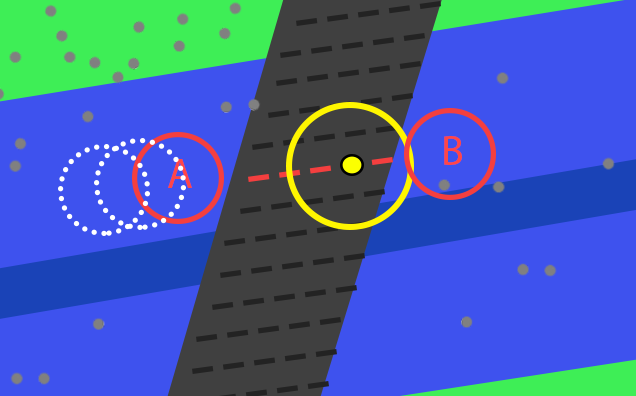
\includegraphics[width=1\columnwidth]{bridge.png}
    \caption{ }
    \label{fig2}
\end{figure}
\begin{itemize}
\item{1. define the bridge polygon from the SHP file and remove every point that is determined to belong to a bridge.}
\item{2. generate values x and y along the bridge in such a way that they run parallel to the valley bellow the bridge. }
\item{3. sample points from both sides of this line (terrain adjecent to the bridge marked with A and B). 
If there are too few points sampled then continue searching in the same direction until some threshold (white dotted circle).
If there are still not enough points to be found sample the surrounging area of the terrain that has already been completed (yellow circle).}
\item{4. Process the sampled points to remove any objects that aren't terrain.}
\item{5. Interpolate the z coordinate with distance as a weight on sampled points.}
\end{itemize}




%TODO: Talk about performance

\section{Bridge reconstruction}




\section{Results}


\begin{figure}[ht]
    \centering
    
\includegraphics[width=1\columnwidth]{side_pre_3.png}
    
\includegraphics[width=1\columnwidth]{side_br_3.png}
    \caption{Results of terrain and bridge reconstruction. Image in yellow shows the original data while the blue image shows the added reconstructed data.}
    \label{fig3}
\end{figure}


\begin{figure}[ht]
    \centering
    
\includegraphics[width=1\columnwidth]{front_pre.png}
    
\includegraphics[width=1\columnwidth]{front_br.png}
    \caption{Results of terrain and bridge reconstruction. Image in yellow shows the original data while the blue image shows the added reconstructed data.}
    \label{fig4}
\end{figure}


\section{Further work}

One of the unsolved problems in our approach is that of saving the reconstructed data in LAZ format.
We weren't sucessful in finding any free library that we could use to save the reconstructed data in the same LAZ format as the input file.
That is why the system outputs a simple OBJ file which contains the reconstructed bridge points alongside with the original points inside of a certain circumference of the bridge.

More of the infrastructure of terrain bellow the bridge could also be supported.
For now only rivers have been supported but also roads, railways or any other kind of infrastructure could be supported as well with the right SHP files and filtering attributes.

\section{Conclusion}

We were sucessful in implementing a rather robust approach for reconstructing bridges and terrain underneath.



%\bibliographystyle{eg-alpha}
\bibliographystyle{eg-alpha-doi}

\bibliography{egbibsample}

\end{document}

